In this section, the training data reduction method for deep learning with support vectors proposed in Section 3 is applied to ResNet 18 ~\cite{bib:Deep-Residual-Learning-for-Image-Recognition}, which is one of the latest neural networks, and evaluation is performed from the viewpoint of training data reduction and classification accuracy. ResNet is one of the networks achieving high accuracy recognition rate in image recognition. We use the CIFAR-10 ~\cite{bib:Convolutional-Deep-Belief-Networks-on-CIFAR-10} data set for evaluation.
\begin{figure}[t]
\begin{center}
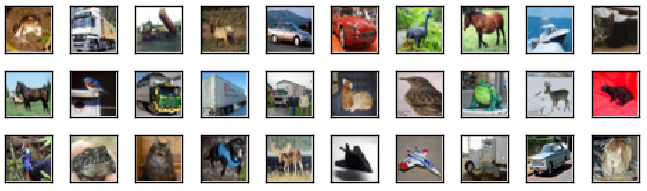
\includegraphics[width=0.95\linewidth]{data/cifar10-2.png}
\end{center}
\caption{A part of CIFAR-10 dataset.}
\vspace*{-3pt}
%{\hfill\footnotesize Note how the caption is centered in the column.\hfill}
\end{figure}

CIFAR-10 is an image data set with a total of 60,000 sheets of 50,000 training data and 10,000 test data.  As shown in Fig. 22, each image is a color image of 3 channels of RGB with $32\times32$ pixels. Each image has a label representing a class, and there are 10 types of class labels: airplane, car, bird, cat, deer, dog, frog, horse, ship, and truck. In this case, two patterns, one for classifying 5 labels, and the other for classifying all 10 labels, are performed. The five labels used for classification are airplanes, birds, deer, frogs and, ships. In all cases, the number of learnings is 100 epochs.

In multiclass classification, since different support vectors are selected for one-to-one classifier and one-to-many classifier, we evaluate both multiclass classification identifications ~\cite{bib:Multi-class-Support-Vector-Machines}. In the one-to-one classifier, ${}_N C _2$ classifiers are used to classify $N$ classes from class $C_1$ to class $C_N$. One-to-many classifiers use N classifiers that solve the two-class classification problem: whether the classification of N classes is classified into a specific class or any other class. 

In the evaluation, we confirme the relationship between classification accuracy and learning time for three cases (A) when using all training data, (B-1) when using only support vectors in a one-to-one classifier and (B-2) when using only support vectors in a one-to-many classifier. Table 3 shows the experimental results for five classes. Table 3 shows that the proposed method reduces the calculation time while achieving the same classification accuracy as the previous method using all the training data. For example, focusing on the calculation accuracy, the calculation accuracy of (A) is 78.300\%, while the calculation accuracy of (B-1) is 78.580\% and (B-2) is 78.340\%, respectively. As for the calculation time, (A) requires 1058.243 seconds for learning, while (B-1) require 961.395 seconds and (B-2) requires 957.629 seconds. In other words, using only the support vector reduced the calculation time by 9.16\% ($1-961.365\div1058.243$) in (B-1) and by 9.50\% ($1-957.629\div1058.243$) in (B-2). Table 4 shows the experimental results for 10 classes. Similar to the evaluation for five classes, the proposed method reduced the calculation time while maintaining the same calculation accuracy as the conventional method. According to Table 4, the calculation time was reduced by 2.54\% ($1-2062.906\div2116.688$) in (B-1) and by 2.66\% ($1-2060.405\div2116.688$) in (B-2). From the above, we confirmed experimentally that the proposed method can reduce the amount of calculation without degradation in accuracy in both 5 label and 10 label evaluations.

It can be read that the reduction effect of calculation time at 10 labels is lower than the effect at 5 labels comparing Table 3 and Table 4. The proposed method reduces the number of data required for training by using only supporter vectors, which is considered to contribute to the reduction of execution results. Focusing on the number of training data required by the conventional method, (B-1) and (B-2), according to Table 3, the number of data is reduced by 11.86\% ($1-22,035\div25,000$) in (B-1) and 12\% ($1-21,975\div25,000$) in (B-2) at 5 labels, respectively. Similarly, according to Table 4, the reduction rate of the number of training data at 10 labels is 4.26\% ($1-47,870\div50,000$) and 4.40\% ($1-47,799\div50,000$). Similar to the reduction rate of calculation time, it can be read that the reduction rate of the number of training data at 5 labels is higher than at 10 labels. 

Based on the above experimental results, we consider training data reduction when using support vectors for CIFAR-10. The preliminary experiments in Section 3.2 reduced the original data by 86 to 88\% when determining the support vector. However, when the support vector was extracted from the training data of CIFAR-10, it was only reduced by about 12\% of the original data in the case of 5 labels. It accounted for a large proportion of the original data and did not provide the expected results from the preliminary experiments in terms of reduction of training data. The cause of this problem is that the problem of identifying color images is much more complicated than that of the preliminary experiments. In the case of a relatively simple data set as treated in the preliminary experiment, no deterioration in accuracy was observed even if the number of data extracted as support vectors was 12 to 14\%. However, in the case of relatively complex data sets such as CIFAR-10, as there are many data responsible for the formation of the classification plane, the number of training data extracted as support vectors is about 88\%, which is the majority of the whole. Compared with the results of the preliminary experiments, although it did not reduce the training data as expected, the training data could be reliably reduced. Moreover, since the accuracy has hardly been deteriorated, it is possible to improve the trade-off between the number of training data and the classification accuracy and to reduce the training data of CIFAR-10 without causing the accuracy deterioration by using the support vector. Compared with the results of the random sampling data performed as a control experiment, the accuracy is also improved, although it is about 1\%. Also, the time taken for learning decreased with the reduction of training data, and it can be said that this was also effective. There were more data extracted as support vectors for 10 labels than for 5 labels, and about 95\% was extracted. Although only 5\%, this was also able to reduce training data. As in the case of 5 labels, almost no degradation in accuracy occurs, so it can be said that the effect of the support vector has been confirmed.

\begin{table}[b]
\begin{center}
\begin{threeparttable}
\caption{Result of applying support vector for CIFAR-10 (5 labels)}
\begin{tabular}{|l|r|c|r|} \hline
training data & data & accuracy(\%) & time(sec) \\ \hline\hline
(A) all data & 25,000 & 78.300 &1058.243 \\ \hline
(B-1) support vector(one-to-one) & 22,035 & 78.580 & 961.394 \\ \hline
(B-2) support vector(one-to-many) & 21,975 & 78.340 & 957.629 \\ \hline
(C-1) random & 22,035 & 77.400 & 962.348 \\ \hline
(C-2) random & 21,975 & 77.260 & 959.526 \\ \hline
\end{tabular}
%\begin{tablenotes}
%\item[a] Uppercase
%\end{tablenotes}
\end{threeparttable}
\end{center}
\end{table}

\begin{table}[b]
\begin{center}
\begin{threeparttable}
\caption{Result of applying support vector for CIFAR-10 (5 labels)}
\begin{tabular}{|l|r|c|r|} \hline
training data & data & accuracy(\%) & time(sec) \\ \hline\hline
(A) all data & 50,000 & 77.560 & 2116.688 \\ \hline
(B-1) support vector(one-to-one) & 47,870 & 77.420 & 2062.906 \\ \hline
(B-2) support vector(one-to-many) & 47,799 & 76.970 & 2060.405 \\ \hline
(C-1) random & 47,870 & 76.580 & 2052.179 \\ \hline
(C-2) random & 47,799 & 76.290 & 2057.681 \\ \hline
\end{tabular}
%\begin{tablenotes}
%\item[a] Uppercase
%\end{tablenotes}
\end{threeparttable}
\end{center}
\end{table}




